\documentclass[conference]{IEEEtran}
\IEEEoverridecommandlockouts

\usepackage[utf8]{inputenc}
\usepackage[T1]{fontenc}
\usepackage[brazil]{babel}
\usepackage{cite}
\usepackage{amsmath,amssymb,amsfonts}
\usepackage{graphicx}
\usepackage{textcomp}
\usepackage{xcolor}
\usepackage{url}
\usepackage{booktabs}
\usepackage{array}
\usepackage{listings}
\usepackage{balance}

% ----- Estilos de código -----
\definecolor{codebg}{RGB}{248,248,248}
\definecolor{codekw}{RGB}{0,73,122}
\definecolor{codecm}{RGB}{82,110,72}
\definecolor{codestr}{RGB}{150,60,40}

\lstdefinestyle{homescript}{
  backgroundcolor=\color{codebg},
  basicstyle=\ttfamily\scriptsize,
  keywordstyle=\color{codekw}\bfseries,
  commentstyle=\color{codecm}\itshape,
  stringstyle=\color{codestr},
  numbers=left, numberstyle=\tiny\color{gray}, numbersep=5pt,
  frame=single, breaklines=true, columns=fullflexible,
  keepspaces=true, showstringspaces=false, tabsize=2,
  morekeywords={device,sensor,pin,type,trig,echo,turn,on,off,wait,
    if,else,for,while,when,detected,not_detected,let,print,
    dispositivo,pino,tipo,gatilho,eco,ligar,desligar,esperar,
    se,senao,para,enquanto,quando,detectado,nao_detectado}
}

\lstdefinestyle{csmall}{
  backgroundcolor=\color{codebg}, language=C,
  basicstyle=\ttfamily\scriptsize,
  keywordstyle=\color{codekw}\bfseries,
  commentstyle=\color{codecm}\itshape,
  numbers=left, numberstyle=\tiny\color{gray}, numbersep=5pt,
  frame=single, breaklines=true, columns=fullflexible,
  keepspaces=true, showstringspaces=false, tabsize=2
}

\lstdefinestyle{plain}{
  backgroundcolor=\color{codebg},
  basicstyle=\ttfamily\scriptsize,
  frame=single, breaklines=true, columns=fullflexible,
  keepspaces=true, showstringspaces=false, tabsize=2
}

\def\BibTeX{{\rm B\kern-.05em{\sc i\kern-.025em b}\kern-.08em
    T\kern-.1667em\lower.7ex\hbox{E}\kern-.125emX}}

\begin{document}

\title{HomeScript: Projeto e Implementação de uma Linguagem de\\
Domínio Específico e seu Compilador para Automação\\
Residencial com Geração de Código C/Arduino}

\author{
\IEEEauthorblockN{Enzo Perroni}
\IEEEauthorblockA{Ciência da Computação\\IBMEC Rio de Janeiro\\Rio de Janeiro, Brasil}
\and
\IEEEauthorblockN{João Pedro Giovanelli}
\IEEEauthorblockA{Ciência da Computação\\IBMEC Rio de Janeiro\\Rio de Janeiro, Brasil}
\and
\IEEEauthorblockN{Arthur Schiller}
\IEEEauthorblockA{Ciência da Computação\\IBMEC Rio de Janeiro\\Rio de Janeiro, Brasil}
\and
\IEEEauthorblockN{Arthur Camaz}
\IEEEauthorblockA{Ciência da Computação\\IBMEC Rio de Janeiro\\Rio de Janeiro, Brasil}
\and
\IEEEauthorblockN{Maria Claudia}
\IEEEauthorblockA{Ciência da Computação\\IBMEC Rio de Janeiro\\Rio de Janeiro, Brasil}
}

\maketitle

% =======================================================
\begin{abstract}
Configurar uma única regra de automação residencial em Arduino --- algo
tão corriqueiro quanto ``acender a luz quando houver movimento'' ---
exige, na prática, escrever código C/C++, declarar pinos, escolher entre
\texttt{digitalRead} e \texttt{analogRead}, inicializar bibliotecas de
sensores e estruturar manualmente \texttt{setup()} e \texttt{loop()}. Quem
sabe \emph{o que} quer automatizar quase nunca sabe \emph{como} o hardware
faz aquilo --- e essa distância afasta o usuário do seu próprio projeto.
Este artigo apresenta o \textbf{HomeScript}: uma linguagem de domínio
específico (DSL) bilíngue (inglês e português) e um compilador completo,
escrito do zero em C, que traduz arquivos \texttt{.iot} em código
C/Arduino pronto para gravar na placa. O compilador percorre as quatro
fases canônicas de um compilador --- análise léxica com 39 classes de
tokens, análise sintática por \emph{parser} recursivo descendente com
construção de Árvore Sintática Abstrata (AST), análise semântica com
tabela de símbolos e escopos aninhados, e geração de código com suporte
nativo aos sensores DHT11 e HC-SR04 --- sem recorrer a geradores
automáticos como Lex/Yacc ou ANTLR. Em torno do compilador construímos um
ecossistema utilizável: uma interface de linha de comando com saída JSON
estruturada, um \emph{backend} REST em FastAPI e uma IDE web em React com
o editor Monaco, autocompletar específico da linguagem, rastreamento
passo a passo do \emph{pipeline} e um construtor visual de automações. A
validação foi conduzida de ponta a ponta: o programa mais abrangente do
repositório (\texttt{casa\_completa\_plus.iot}), com 9 atuadores e 6
sensores, foi compilado e o código C resultante gravado \emph{sem
edição manual} em um Arduino Uno (ATMega328P) físico, reproduzindo
fielmente o comportamento descrito na linguagem. O resultado demonstra
que uma DSL pequena e bem direcionada pode esconder a complexidade do
baixo nível e, ao mesmo tempo, servir de veículo didático para todas as
fases clássicas da construção de compiladores.
\end{abstract}

\begin{IEEEkeywords}
Compiladores, linguagens de domínio específico, automação residencial,
sistemas embarcados, geração de código, microcontroladores.
\end{IEEEkeywords}

% =======================================================
\section{Introdução}
\label{sec:intro}

\subsection{Contexto: automação residencial e a Internet das Coisas}

A automação residencial deixou de ser um nicho de entusiastas e tornou-se
um dos segmentos de maior crescimento da Internet das Coisas
(IoT)~\cite{atzori2010,alfuqaha2015,gubbi2013}. Projeções recorrentes na
literatura estimam dezenas de bilhões de dispositivos conectados em
operação ao longo desta década~\cite{zanella2014}, abrangendo desde o
simples controle de iluminação até sistemas integrados de segurança,
climatização, irrigação e gerenciamento de energia. No coração de boa
parte desses projetos --- sobretudo na fase de prototipagem e no contexto
educacional --- está a plataforma Arduino~\cite{banzi2011}, que se
consolidou como padrão de fato graças ao baixo custo, ao ecossistema
maduro de bibliotecas e a uma comunidade ampla.

\subsection{O problema: a barreira da programação embarcada}

Apesar da popularidade do Arduino, a distância entre \emph{descrever} uma
automação e \emph{implementá-la} permanece grande. Considere a regra
trivial ``ligar uma lâmpada quando um sensor detectar movimento''. Para
realizá-la, o programador precisa: declarar o pino da lâmpada como
\texttt{OUTPUT} com \texttt{pinMode}; configurar o pino do sensor como
\texttt{INPUT}; chamar \texttt{digitalRead} dentro do \texttt{loop()};
comparar o valor lido com \texttt{HIGH}; e, só então, invocar
\texttt{digitalWrite}. Quando entram em cena sensores especializados, a
complexidade cresce de forma desproporcional ao objetivo: o DHT11
(temperatura e umidade) requer biblioteca externa, instanciação de objeto
e tratamento de leituras inválidas (\texttt{NaN}); o ultrassônico HC-SR04
exige a geração manual de um pulso de disparo e a medição do tempo de eco
com \texttt{pulseIn}, além da conversão do tempo em distância. Em outras
palavras, há um descompasso entre a \emph{intenção} (uma regra de
negócio simples) e a \emph{implementação} (dezenas de detalhes elétricos
e de API). Esse descompasso é exatamente o tipo de problema que uma
linguagem de domínio específico se propõe a resolver.

\subsection{O que é um compilador e por que construir um}

Um \emph{compilador} é um programa que traduz texto escrito em uma
linguagem-fonte para uma linguagem-alvo, preservando o significado do
programa~\cite{aho2006,cooper2011}. Diferentemente de um interpretador,
que executa o programa diretamente, o compilador produz um artefato
intermediário --- no nosso caso, código C/Arduino --- que será, por sua
vez, compilado e executado em outro ambiente. A construção de
compiladores é tradicionalmente organizada em fases bem
definidas~\cite{aho2006,grune2012,appel1998}: a \emph{análise} (front-end)
decompõe o texto em \emph{tokens} (análise léxica), reconhece sua
estrutura gramatical (análise sintática) e verifica sua coerência lógica
(análise semântica); a \emph{síntese} (back-end) gera o código de saída a
partir de uma representação intermediária. Essa separação não é apenas
teórica: ela orienta a engenharia do software, pois cada fase possui
entrada e saída bem delimitadas, podendo ser testada, depurada e
explicada isoladamente.

A teoria que fundamenta essas fases é madura. O reconhecimento de tokens
apoia-se em expressões regulares e autômatos finitos; a análise sintática,
em gramáticas livres de contexto e técnicas de \emph{parsing} como a
descida recursiva (\emph{recursive descent})~\cite{wirth1976}. Ferramentas
de geração automática como Lex/Yacc e ANTLR~\cite{parr2013} produzem
\emph{lexers} e \emph{parsers} a partir de especificações declarativas.
Optamos deliberadamente por \emph{não} usá-las: implementar cada fase
manualmente, em C, expõe o funcionamento interno do \emph{pipeline} e
constitui o cerne do exercício acadêmico que motivou este trabalho.

\subsection{A ideia e a pesquisa: por que uma DSL}

A ideia do HomeScript surgiu da observação de que regras de automação
residencial compartilham uma estrutura repetitiva: há \emph{entradas}
(sensores), \emph{saídas} (atuadores), \emph{condições} e \emph{ações}.
Em vez de exigir que cada usuário reescreva manualmente o mesmo padrão de
código Arduino, é possível encapsular esse padrão em uma linguagem.

Linguagens de domínio específico (DSLs) são a resposta consolidada para
esse tipo de problema~\cite{mernik2005,fowler2010,vandeursen2000}. Ao
contrário de linguagens de propósito geral, uma DSL restringe o espaço de
expressão ao conjunto de conceitos relevantes para um domínio, tornando os
programas mais curtos, mais legíveis e menos suscetíveis a erros de baixo
nível. SQL (consultas a bancos de dados), HTML (estrutura de documentos) e
VHDL (descrição de hardware) são exemplos canônicos do quanto uma boa DSL
pode aproximar a linguagem da intenção do usuário. A pesquisa inicial da
equipe consolidou três requisitos, alinhados aos critérios de Mernik et
al.~\cite{mernik2005} para o desenvolvimento de DSLs: \textbf{(i)}
proximidade com a linguagem natural, para que comandos sejam
compreensíveis sem documentação; \textbf{(ii)} correspondência direta e
não ambígua com operações de hardware do Arduino~\cite{arduino2024}; e
\textbf{(iii)} viabilidade de implementação completa dentro de um
compilador escrito em C.

\subsection{Objetivos e contribuições}

O HomeScript foi concebido com um \emph{objetivo duplo}, que permeia todas
as decisões de projeto descritas neste artigo:

\begin{itemize}
\item \textbf{Objetivo acadêmico:} implementar, a partir dos fundamentos,
um compilador completo com todas as fases canônicas --- léxica,
sintática, semântica e geração de código --- demonstrando na prática os
conceitos da disciplina.
\item \textbf{Objetivo de produto:} oferecer uma ferramenta genuinamente
utilizável, com interface web, autocompletar, construtor visual e suporte
bilíngue, capaz de gerar código Arduino correto a partir de uma descrição
declarativa.
\end{itemize}

A Listagem~\ref{lst:intro} ilustra uma automação básica em HomeScript: o
compilador transforma esse arquivo em código C completo --- com
\texttt{setup()}, \texttt{loop()}, \texttt{pinMode} e \texttt{digitalRead}
--- sem que o usuário precise conhecer qualquer um desses detalhes.

\begin{lstlisting}[style=homescript,caption={Automação básica em HomeScript.},label={lst:intro}]
device luz pin 13;
sensor movimento pin 2;

when movimento == detected {
    turn luz on;
    wait 5000;
    turn luz off;
}
\end{lstlisting}

\subsection{Organização do artigo}

O restante do texto está organizado em torno de cinco eixos macro. A
Seção~\ref{sec:linguagem} define a linguagem HomeScript e seus princípios
de design. A Seção~\ref{sec:compilador} descreve, passo a passo, o
desenvolvimento do compilador e a implementação de cada uma de suas quatro
fases. A Seção~\ref{sec:sistema} apresenta o sistema integrado --- CLI,
\emph{backend} e a IDE web --- isto é, a aplicação que torna o compilador
um produto. A Seção~\ref{sec:validacao} relata a validação de ponta a
ponta com hardware físico, analisando o código gerado e discutindo os
acertos, erros e estratégias de depuração do projeto. A
Seção~\ref{sec:conclusao} conclui e aponta trabalhos futuros.

% =======================================================
\section{A Linguagem HomeScript}
\label{sec:linguagem}

\subsection{Princípios de design}

A definição da linguagem partiu dos três requisitos levantados na pesquisa
(Seção~\ref{sec:intro}) e os converteu em decisões concretas:

\begin{enumerate}
\item \textbf{Proximidade com a linguagem natural.} Comandos como
\texttt{turn luz on} e \texttt{wait 1000} foram escolhidos para serem
autoexplicativos. A pontuação é mínima: comandos terminam em ponto e
vírgula e blocos são delimitados por chaves.
\item \textbf{Correspondência direta com o hardware.} Cada construção da
linguagem mapeia para uma chamada Arduino bem definida, sem ambiguidade ---
\texttt{turn} vira \texttt{digitalWrite}, \texttt{wait} vira
\texttt{delay}, e assim por diante.
\item \textbf{Bilinguismo nativo.} Palavras-chave em português são tratadas
como sinônimos \emph{no nível léxico}, sem qualquer impacto sobre o
\emph{parser} ou o gerador. Isso aproxima a linguagem do público
brasileiro sem duplicar a gramática.
\end{enumerate}

Arquivos HomeScript usam texto UTF-8 com extensão \texttt{.iot} e admitem
comentários de linha iniciados por \texttt{//}.

\subsection{Declarações de hardware}

\subsubsection{Dispositivos}
Representam atuadores digitais (lâmpadas, ventiladores, sirenes, motores).
A declaração \texttt{device <nome> pin <N>;} gera, no código de saída,
\texttt{\#define <nome> <N>} e o respectivo \texttt{pinMode(<nome>, OUTPUT)}.
A forma em português usa \texttt{dispositivo}/\texttt{pino}.

\subsubsection{Sensores}
A linguagem reconhece quatro categorias de sensor, cada uma com tradução
distinta para C:
\begin{itemize}
\item \textbf{Digital genérico} (\texttt{pin N}): lido com
\texttt{digitalRead}; comparado com \texttt{detected}/\texttt{not\_detected}.
\item \textbf{Analógico} (\texttt{pin AN}): lido com \texttt{analogRead};
comparações obrigatoriamente numéricas.
\item \textbf{DHT11} (\texttt{type dht11 pin N}): gera um objeto
\texttt{DHT}, leitura via \texttt{readTemperature()} protegida por
\texttt{!isnan()}.
\item \textbf{HC-SR04} (\texttt{type hcsr04 trig N echo N}): gera uma
função auxiliar que dispara o pulso e mede o eco com \texttt{pulseIn}.
\end{itemize}

Vale destacar uma nuance de design: as palavras \texttt{type}/\texttt{tipo},
\texttt{trig}/\texttt{gatilho} e \texttt{echo}/\texttt{eco} \emph{não} são
palavras reservadas. Elas são reconhecidas \emph{contextualmente} pelo
\emph{parser} apenas dentro da declaração de sensores, o que mantém o
conjunto de palavras-chave enxuto e evita ``roubar'' esses nomes do espaço
de identificadores do usuário.

\subsection{Variáveis e expressões}

Variáveis inteiras são declaradas com \texttt{let <nome> = <expr>;}. As
expressões aritméticas suportam os operadores \texttt{+}, \texttt{-},
\texttt{*} e \texttt{/}, com a precedência convencional (multiplicação e
divisão antes de soma e subtração) e agrupamento por parênteses. As
variáveis são traduzidas para inteiros globais (\texttt{int}) em C.

\subsection{Estruturas de controle}
\label{subsec:controle}

A linguagem oferece dois condicionais e dois laços:
\texttt{if}/\texttt{se} e \texttt{when}/\texttt{quando} aceitam uma
condição, um bloco obrigatório e um bloco \texttt{else}/\texttt{senao}
opcional; os laços \texttt{while}/\texttt{enquanto} e
\texttt{for}/\texttt{para} aceitam tanto variáveis quanto sensores na
condição, reavaliada a cada iteração. A Listagem~\ref{lst:controle} mostra
um trecho com laço aninhado e \texttt{senao}.

\begin{lstlisting}[style=homescript,caption={Estruturas de controle e bilinguismo.},label={lst:controle}]
quando porta_entrada == detectado {
    contador_alertas = contador_alertas + 1;
    ligar luz_corredor;
    para i = 0; i < 3; i = i + 1 {
        ligar sirene;  esperar 250;
        desligar sirene;  esperar 250;
    }
} senao {
    desligar luz_corredor;
}
\end{lstlisting}

\subsection{Sistema de tokens}

O analisador léxico reconhece \textbf{39 classes de tokens}. As palavras
reservadas somam 28 entradas --- 16 em inglês (\texttt{device}, \texttt{sensor},
\texttt{pin}, \texttt{let}, \texttt{print}, \texttt{turn}, \texttt{on},
\texttt{off}, \texttt{wait}, \texttt{if}, \texttt{for}, \texttt{while},
\texttt{else}, \texttt{when}, \texttt{detected}, \texttt{not\_detected}) e
12 em português, que reaproveitam os mesmos tipos de token. A
Tabela~\ref{tab:tokens} resume as categorias principais.

\begin{table}[htbp]
\caption{Classes de tokens da linguagem HomeScript}
\label{tab:tokens}
\centering
\begin{tabular}{p{0.21\linewidth}p{0.20\linewidth}p{0.47\linewidth}}
\toprule
\textbf{Categoria} & \textbf{Exemplos} & \textbf{Padrão / regra} \\
\midrule
Palavra-chave EN & \texttt{device}, \texttt{when} & Verificação após identificador \\
Palavra-chave PT & \texttt{dispositivo}, \texttt{quando} & Mesmo mecanismo \\
Identificador & \texttt{luz}, \texttt{temp1} & \texttt{[a-zA-Z\_][a-zA-Z0-9\_]*} \\
Número & \texttt{13}, \texttt{1000} & \texttt{[0-9]+} \\
Pino analógico & \texttt{A0}, \texttt{A1} & \texttt{A[0-9]+} (prioridade) \\
Op. relacional & \texttt{==}, \texttt{!=}, \texttt{>=} & \emph{Lookahead} de 1 caractere \\
Op. aritmético & \texttt{+}, \texttt{-}, \texttt{*}, \texttt{/} & Caractere único \\
Delimitadores & \texttt{\{}, \texttt{\}}, \texttt{;}, \texttt{(}, \texttt{)} & Caractere único \\
Especiais & \texttt{EOF}, erro & Fim de arquivo / caractere inválido \\
\bottomrule
\end{tabular}
\end{table}

% =======================================================
\section{Desenvolvimento do Compilador}
\label{sec:compilador}

\subsection{Metodologia incremental}

O compilador não foi escrito de uma só vez. A equipe adotou uma
abordagem \emph{incremental}, em que cada fase era construída, testada e
demonstrada antes de ser conectada ao restante do \emph{pipeline}. Essa
decisão reduziu o risco e facilitou a depuração: primeiro definiu-se a
especificação da linguagem (exemplos \texttt{.iot}, tabela de tokens e
expressões regulares); em seguida implementou-se o \emph{lexer}; depois o
\emph{parser} com a AST; então o gerador de código; e, por fim, a análise
semântica --- adicionada quando ficou evidente que um programa
sintaticamente correto ainda podia ser logicamente inválido. A integração
com \emph{backend} e \emph{frontend} veio por último, sem alterar o
compilador. Cada novo recurso da linguagem (variáveis, laços, sensores
especializados) foi acompanhado de um exemplo concreto que servia
simultaneamente de teste e de documentação.

\subsection{Visão geral da arquitetura em fases}

O compilador foi implementado integralmente em C (padrão C99), sem
dependências externas, e organizado em quatro módulos independentes ---
\texttt{lexer/}, \texttt{parser/} (com a AST), \texttt{semantic/} e
\texttt{codegen/} --- integrados pelo executável \texttt{compiler/main.c}.
A Tabela~\ref{tab:modulos} resume a responsabilidade de cada módulo. O
fluxo de dados é estritamente unidirecional, como ilustra a
Fig.~\ref{fig:ide} (que também mostra o resultado dessas fases na IDE):
texto \texttt{.iot} $\rightarrow$ tokens $\rightarrow$ AST $\rightarrow$
verificação semântica $\rightarrow$ código C.

\begin{table}[htbp]
\caption{Módulos do compilador e suas responsabilidades}
\label{tab:modulos}
\centering
\begin{tabular}{p{0.20\linewidth}p{0.70\linewidth}}
\toprule
\textbf{Módulo} & \textbf{Responsabilidade} \\
\midrule
\texttt{lexer/} & Reconhecimento de tokens, controle de linha/coluna, comentários e erros léxicos. \\
\texttt{parser/} & \emph{Parser} recursivo descendente, definição e construção da AST, impressão e serialização. \\
\texttt{semantic/} & Tabela de símbolos, escopos aninhados, validação de dispositivos, sensores, variáveis e pinos. \\
\texttt{codegen/} & Tradução da AST para C/Arduino, incluindo sensores DHT11 e HC-SR04 e cache de leituras. \\
\texttt{compiler/} & CLI, orquestração das fases, saída textual e saída JSON. \\
\bottomrule
\end{tabular}
\end{table}

\subsection{Análise léxica}

O \emph{lexer} mantém um estado compacto com quatro campos relevantes:
\texttt{FILE *arquivo}, \texttt{char caractere\_atual}, \texttt{int linha}
e \texttt{int coluna}. Ele lê o arquivo caractere a caractere, sem carregar
todo o conteúdo em memória, e a função central
\texttt{lexer\_proximo\_token()} executa dois passos: primeiro pula
espaços, quebras de linha e comentários de linha (via
\texttt{lexer\_pular\_insignificantes()}); depois examina o caractere
corrente e despacha para a sub-rotina adequada.

Dois pontos merecem destaque. O primeiro é a \emph{prioridade do pino
analógico}: quando o caractere é \texttt{'A'} e o próximo é um dígito, o
\emph{lexer} reconhece um pino analógico (\texttt{A0}, \texttt{A1}, \dots)
\emph{antes} de tentar ler um identificador. O segundo é o uso de
\emph{lookahead} de um caractere (via \texttt{fgetc}/\texttt{ungetc}) para
distinguir operadores simples de compostos: \texttt{=} pode ser atribuição
ou parte de \texttt{==}; \texttt{>} pode compor \texttt{>=}; e \texttt{!}
só é válido quando seguido de \texttt{=}, gerando \texttt{TOKEN\_ERROR}
caso contrário. A Listagem~\ref{lst:lexer} mostra o esqueleto da função.

\begin{lstlisting}[style=csmall,caption={Despacho principal do lexer.},label={lst:lexer}]
Token lexer_proximo_token(Lexer *lexer) {
    lexer_pular_insignificantes(lexer);
    if (lexer->eof)
        return criar_token(TOKEN_EOF, "EOF", ...);

    char c = lexer->caractere_atual;
    if (c=='A' && isdigit(lexer_espiar(lexer)))
        return lexer_ler_pino_analogico(lexer);
    if (isalpha(c) || c=='_')
        return lexer_ler_identificador(lexer);
    if (isdigit(c))
        return lexer_ler_numero(lexer);
    if (c=='='||c=='!'||c=='>'||c=='<')
        return lexer_ler_operador(lexer);
    /* +, -, *, /, {, }, ;, (, ) e erro */
}
\end{lstlisting}

A distinção entre palavra reservada e identificador acontece \emph{a
posteriori}: o \emph{lexer} lê a sequência de letras/dígitos/sublinhados e
só então a compara, em \texttt{verificar\_palavra\_reservada()}, contra a
lista de 28 palavras-chave. Cada token carrega tipo, valor (até 256
caracteres), linha e coluna --- e essa informação de posição percorre todo
o \emph{pipeline}, sendo reaproveitada pelo \emph{parser}, pela saída JSON
e, no \emph{frontend}, para destacar a localização exata dos erros.

\subsection{Análise sintática e a AST}

\subsubsection{Estrutura da AST}
A AST, definida em \texttt{parser/ast.h}, adota uma \emph{representação
uniforme}: todo nó é uma estrutura \texttt{ASTNode} com campos genéricos,
em vez de uma \texttt{struct} distinta para cada construção. Existem
\textbf{14 tipos de nó} (\texttt{NodeType}): \texttt{NODE\_PROGRAM} (raiz),
as declarações (\texttt{DEVICE\_DECL}, \texttt{SENSOR\_DECL},
\texttt{VAR\_DECL}), os comandos (\texttt{ASSIGN\_CMD}, \texttt{PRINT\_CMD},
\texttt{TURN\_CMD}, \texttt{WAIT\_CMD}), as estruturas de controle
(\texttt{IF\_STMT}, \texttt{WHEN\_STMT}, \texttt{FOR\_STMT},
\texttt{WHILE\_STMT}), além de \texttt{BLOCK} e \texttt{CONDITION}. Cada nó
reúne campos como \texttt{nome}, \texttt{pino}, \texttt{pino\_secundario}
(o \texttt{echo} do HC-SR04), \texttt{sensor\_tipo}, \texttt{operador}
(EQ, NE, GT, LT, GE, LE), \texttt{valor\_comparacao}, \texttt{estado}
(ON/OFF), \texttt{tempo\_espera} e \texttt{expressao}, e suporta até 64
filhos. Essa escolha simplifica a implementação ao custo de algum
desperdício de memória por nó --- um trade-off consciente e adequado à
escala da linguagem.

\subsubsection{Parser recursivo descendente}
O \emph{parser} é recursivo descendente (RDP)~\cite{aho2006,wirth1976},
técnica adequada a gramáticas LL(1), nas quais cada produção é determinada
pelo próximo token, sem \emph{backtracking}. A função
\texttt{parser\_analisar()} cria o nó raiz e chama repetidamente
\texttt{parser\_statement()} até o \texttt{EOF}; um despachante baseado em
\texttt{switch} seleciona a função de produção correta para cada token
inicial (Listagem~\ref{lst:parser}).

\begin{lstlisting}[style=csmall,caption={Despachante de comandos do parser.},label={lst:parser}]
static ASTNode* parser_statement(Parser *p) {
    switch (p->token_atual.tipo) {
      case TOKEN_DEVICE:     return parser_device_decl(p);
      case TOKEN_SENSOR:     return parser_sensor_decl(p);
      case TOKEN_LET:        return parser_var_decl(p);
      case TOKEN_PRINT:      return parser_print_cmd(p);
      case TOKEN_TURN:
      case TOKEN_LIGAR:
      case TOKEN_DESLIGAR:   return parser_turn_cmd(p);
      case TOKEN_WAIT:       return parser_wait_cmd(p);
      case TOKEN_IF:         return parser_if_stmt(p);
      case TOKEN_FOR:        return parser_for_stmt(p);
      case TOKEN_WHILE:      return parser_while_stmt(p);
      case TOKEN_WHEN:       return parser_when_stmt(p);
      case TOKEN_IDENTIFIER: return parser_assign_cmd(p);
      case TOKEN_ELSE:
        parser_registrar_erro(p, "else/senao sem if/when");
        return NULL;
      default:
        parser_registrar_erro(p, "Comando nao reconhecido");
        return NULL;
    }
}
\end{lstlisting}

A precedência das expressões aritméticas é codificada na própria
hierarquia de chamadas, padrão clássico de RDP:
\texttt{parser\_expressao()} trata \texttt{+}/\texttt{-} e chama
\texttt{parser\_termo()}, que trata \texttt{*}/\texttt{/} e chama
\texttt{parser\_fator()}, que reconhece números, identificadores e
expressões entre parênteses. Vale registrar uma decisão pragmática: o
resultado de uma expressão é \emph{normalizado e armazenado como texto} no
campo \texttt{expressao} do nó, e não como uma subárvore própria. Isso
simplificou a implementação e a geração de código, mas tem consequências
discutidas na Seção~\ref{subsec:limitacoes}.

Quanto à forma dos nós: um \texttt{for} possui sempre quatro filhos
--- \texttt{[init, cond, update, bloco]}, em que \texttt{init} e
\texttt{update} são reaproveitados do mesmo código de atribuição; os
condicionais possuem dois ou três filhos --- \texttt{[cond, then]} ou
\texttt{[cond, then, else]}. O \emph{parser} adota a estratégia
\emph{stop-on-first-error}: ao primeiro erro, registra mensagem com fase,
linha, coluna e o token efetivamente encontrado, e interrompe a análise.
Entre os erros tratados estão a ausência de \texttt{;}, o bloco não
fechado, o comando desconhecido, o \texttt{else} órfão e o token inválido
herdado do \emph{lexer}.

\subsection{Análise semântica}

A análise semântica (\texttt{semantic/semantic.c}) foi a última fase a ser
adicionada e é a que separa um programa \emph{sintaticamente} correto de um
programa \emph{logicamente} correto. Ela mantém uma tabela de símbolos com
até 256 entradas e até 64 escopos aninhados, e opera em dois passos sobre
a AST. O primeiro, \texttt{coletar\_declaracoes\_fixas()}, percorre toda a
árvore e registra globalmente todos os dispositivos e sensores --- o que
permite que uma regra referencie um dispositivo independentemente da ordem
de declaração. O segundo, \texttt{analisar\_no()}, percorre a AST validando
cada nó e gerenciando o escopo das variáveis com \texttt{push\_scope()} e
\texttt{pop\_scope()} ao entrar e sair de blocos. As verificações
implementadas são:

\begin{itemize}
\item identificadores duplicados no mesmo escopo;
\item conflito de pinos entre dispositivos e sensores;
\item \texttt{trig} e \texttt{echo} iguais em um HC-SR04;
\item uso de dispositivo não declarado em \texttt{turn}/\texttt{ligar}/\texttt{desligar};
\item uso de sensor inexistente na condição de \texttt{if}/\texttt{when};
\item comparação de um DHT11 com \texttt{detected} --- um erro de tipo
semântico, pois esse sensor exige comparação numérica;
\item atribuição a uma variável não declarada;
\item identificador desconhecido dentro de uma expressão aritmética;
\item valor de condição que não é número, palavra reservada nem variável
visível.
\end{itemize}

Sem essa fase, um comando como \texttt{turn bomba on;} sobre uma
\texttt{bomba} não declarada geraria \texttt{digitalWrite(bomba, HIGH)} ---
um erro que só apareceria, de forma obscura, no compilador do Arduino. Com
a verificação semântica, o erro é reportado diretamente na linguagem
HomeScript, com linha e coluna.

\subsection{Geração de código C/Arduino}

O gerador (\texttt{codegen/codegen.c}) acumula o código de saída em um
\emph{buffer} estático de 8.192 bytes e o organiza em três partes:
preâmbulo, \texttt{setup()} e \texttt{loop()}.

No \textbf{preâmbulo}, dispositivos viram macros \texttt{\#define}; sensores
genéricos viram variáveis de pino (\texttt{int <nome>\_pin = N;}); o DHT11
instancia o objeto \texttt{DHT} e provoca a inclusão de \texttt{<DHT.h>}; o
HC-SR04 gera dois inteiros de pino e uma função auxiliar de medição; e as
variáveis \texttt{let} viram inteiros globais. A função \texttt{setup()}
emite os \texttt{pinMode} apropriados (\texttt{OUTPUT} para atuadores,
\texttt{INPUT} para sensores), o \texttt{begin()} do DHT11, a configuração
de \texttt{trig}/\texttt{echo} do HC-SR04 e, sempre,
\texttt{Serial.begin(9600)}.

A tradução de \emph{condições} depende do tipo do sensor: digital com
\texttt{detected} vira \texttt{digitalRead(pin) == HIGH}; analógico vira
\texttt{analogRead(pin) op valor}; DHT11 vira
\texttt{!isnan(leit) \&\& leit op valor}; e HC-SR04 invoca a função
auxiliar. Os laços \texttt{while} e \texttt{for} adotam o padrão da
Listagem~\ref{lst:loop}, que reavalia a condição (e, portanto, relê o
sensor) a cada iteração sem duplicar código.

\begin{lstlisting}[style=csmall,caption={Padrão de geração de laços.},label={lst:loop}]
while (1) {
    if (!(condicao)) break;
    /* corpo do laco */
}
\end{lstlisting}

A otimização mais interessante do gerador é o \textbf{cache de leituras}.
Quando um bloco \texttt{if}/\texttt{else} e o seu \texttt{else} imediato
referenciam o \emph{mesmo} sensor, o gerador materializa uma única variável
temporária antes do \texttt{if} e a reutiliza em ambos os ramos. A detecção
verifica se o primeiro filho do bloco \texttt{else} é, ele próprio, um
\texttt{if}/\texttt{when} sobre o mesmo sensor. Isso é decisivo para
sensores lentos como o DHT11, cuja leitura custa centenas de
milissegundos: sem o cache, um \texttt{if/else} aninhado faria duas
chamadas a \texttt{readTemperature()} por ciclo do \texttt{loop()}. O
efeito desse mecanismo é analisado em detalhe na
Seção~\ref{subsec:codegen_analise}.

\subsection{Interface de linha de comando e saída JSON}

O executável \texttt{homescript} aceita as opções \texttt{--tokens},
\texttt{--ast}, \texttt{--code}, \texttt{--output <arquivo>} e
\texttt{--json}, além de exibir tudo quando invocado sem opções de filtro.
O modo \texttt{--json} é o que viabiliza a integração com a web: ele produz
um objeto único com os campos \texttt{tokens}, \texttt{sucesso},
\texttt{erro}, \texttt{erros} (um \emph{array} com fase, mensagem, linha e
coluna), \texttt{ast} (serializada recursivamente) e \texttt{codigo\_c}.
Projetar essa saída estruturada \emph{dentro} do compilador foi uma decisão
de arquitetura importante: ela evita que qualquer outra camada precise
interpretar texto formatado para humanos, mantendo o compilador como a
única fonte da verdade.

% =======================================================
\section{Sistema Integrado e a Aplicação}
\label{sec:sistema}

\subsection{Arquitetura de três camadas}

Em torno do compilador foi construído um sistema em três camadas, com
fronteiras deliberadamente nítidas. O \textbf{compilador C} é
autossuficiente como ferramenta de linha de comando. O \textbf{backend
Python} apenas o encapsula via subprocesso. O \textbf{frontend React}
apenas consome a API REST e apresenta os dados. Essa separação garante que
a CLI e a interface web produzam exatamente o mesmo resultado, porque ambas
executam o \emph{mesmo binário} --- não há lógica de compilação duplicada
em Python ou JavaScript.

\subsection{Backend REST}

O \emph{backend} (\texttt{backend/app.py}) usa FastAPI~\cite{fastapi2024} e
expõe os \emph{endpoints} \texttt{POST /compile}, \texttt{POST /tokens},
\texttt{GET /health} e \texttt{GET /exemplos}. A ponte com o compilador
(\texttt{compiler\_bridge.py}) grava o código recebido em um arquivo
temporário \texttt{.iot}, executa \texttt{homescript --json}, captura a
saída-padrão e a interpreta como JSON. Ela trata de forma robusta os três
modos de falha esperados: ausência do binário (\texttt{FileNotFoundError}),
estouro de tempo (\texttt{TimeoutExpired}, com limite de 10 segundos) e
JSON malformado (\texttt{JSONDecodeError}); e remove o arquivo temporário
ao final, mesmo em caso de erro.

\subsection{A IDE web}

O \emph{frontend} usa React, Vite e o editor Monaco~\cite{react2024,monaco2024}.
Foi registrada uma linguagem customizada \texttt{homescript}, com
realce de sintaxe (palavras-chave em inglês e português, comentários,
números, operadores e delimitadores), fechamento automático de blocos e um
provedor de autocompletar com mais de trinta entradas --- incluindo
\emph{snippets} para DHT11, HC-SR04, \texttt{if}/\texttt{when}/\texttt{for}/\texttt{while}
e todos os equivalentes em português. A tela principal (Fig.~\ref{fig:ide})
funciona como uma IDE: o usuário escreve o código, carrega exemplos do
repositório, compila com um botão ou com \texttt{Ctrl/Cmd+Enter} e
inspeciona o resultado em quatro abas.

\begin{figure}[htbp]
\centerline{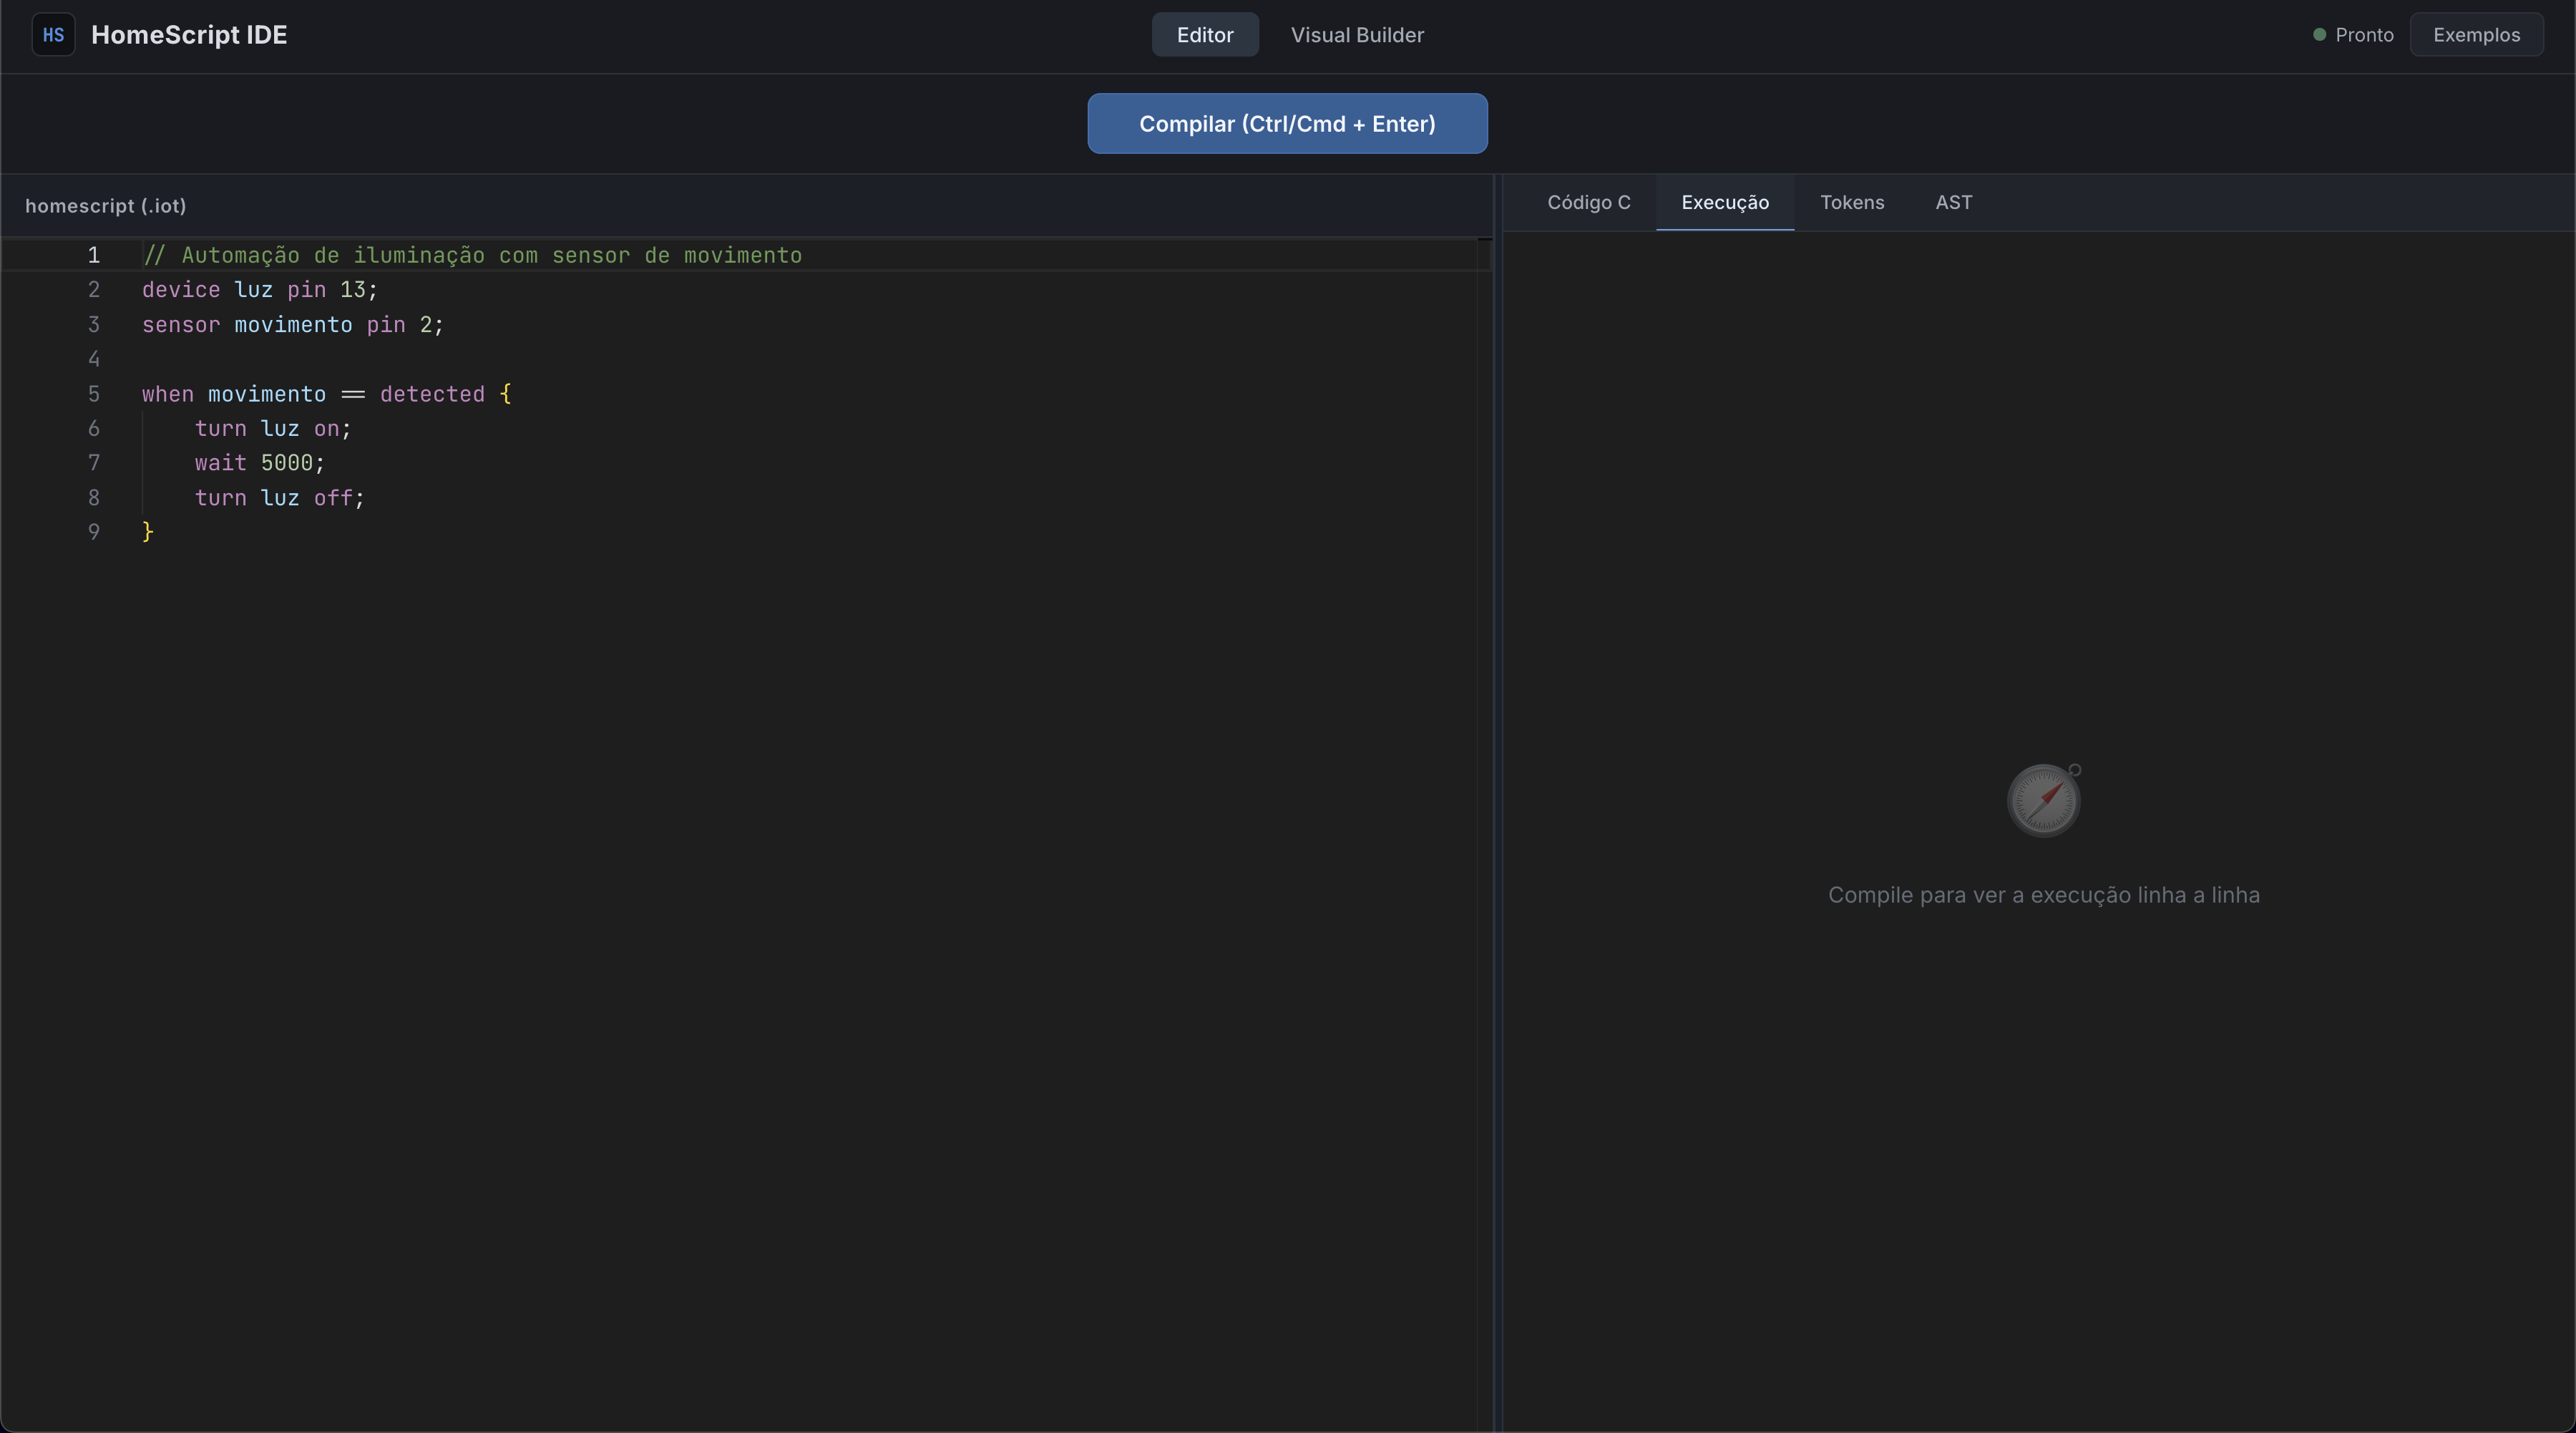
\includegraphics[width=0.95\linewidth]{../img/tela1.png}}
\caption{IDE HomeScript: editor Monaco à esquerda; à direita, painel de resultados com as abas Código C, Execução, Tokens e AST.}
\label{fig:ide}
\end{figure}

As abas são: \textbf{Código C} (com botão de copiar), \textbf{Tokens}
(tipo, valor, linha e coluna de cada token), \textbf{AST} (a árvore
serializada pelo \emph{backend}) e \textbf{Execução}. Esta última é uma
contribuição pedagógica do projeto: ela constrói um rastro passo a passo do
\emph{pipeline}, mostrando, para cada token, a função interna do
\emph{lexer} acionada e os caracteres consumidos --- transformando o
funcionamento normalmente opaco do compilador em uma explicação visual.

\subsection{Construtor visual (Visual Builder)}

Para o usuário que não deseja escrever código, a segunda tela
(Fig.~\ref{fig:visual}) oferece um construtor visual. Nele se cadastram
dispositivos e sensores em formulários e se montam regras no formato
``\texttt{QUANDO} sensor operador valor $\rightarrow$ dispositivo estado
(\emph{wait} opcional)''. Ao confirmar, a interface \emph{gera código
HomeScript válido} e o devolve ao editor textual, fechando o ciclo entre a
experiência de produto (montar visualmente) e o núcleo acadêmico (compilar
de verdade).

\begin{figure}[htbp]
\centerline{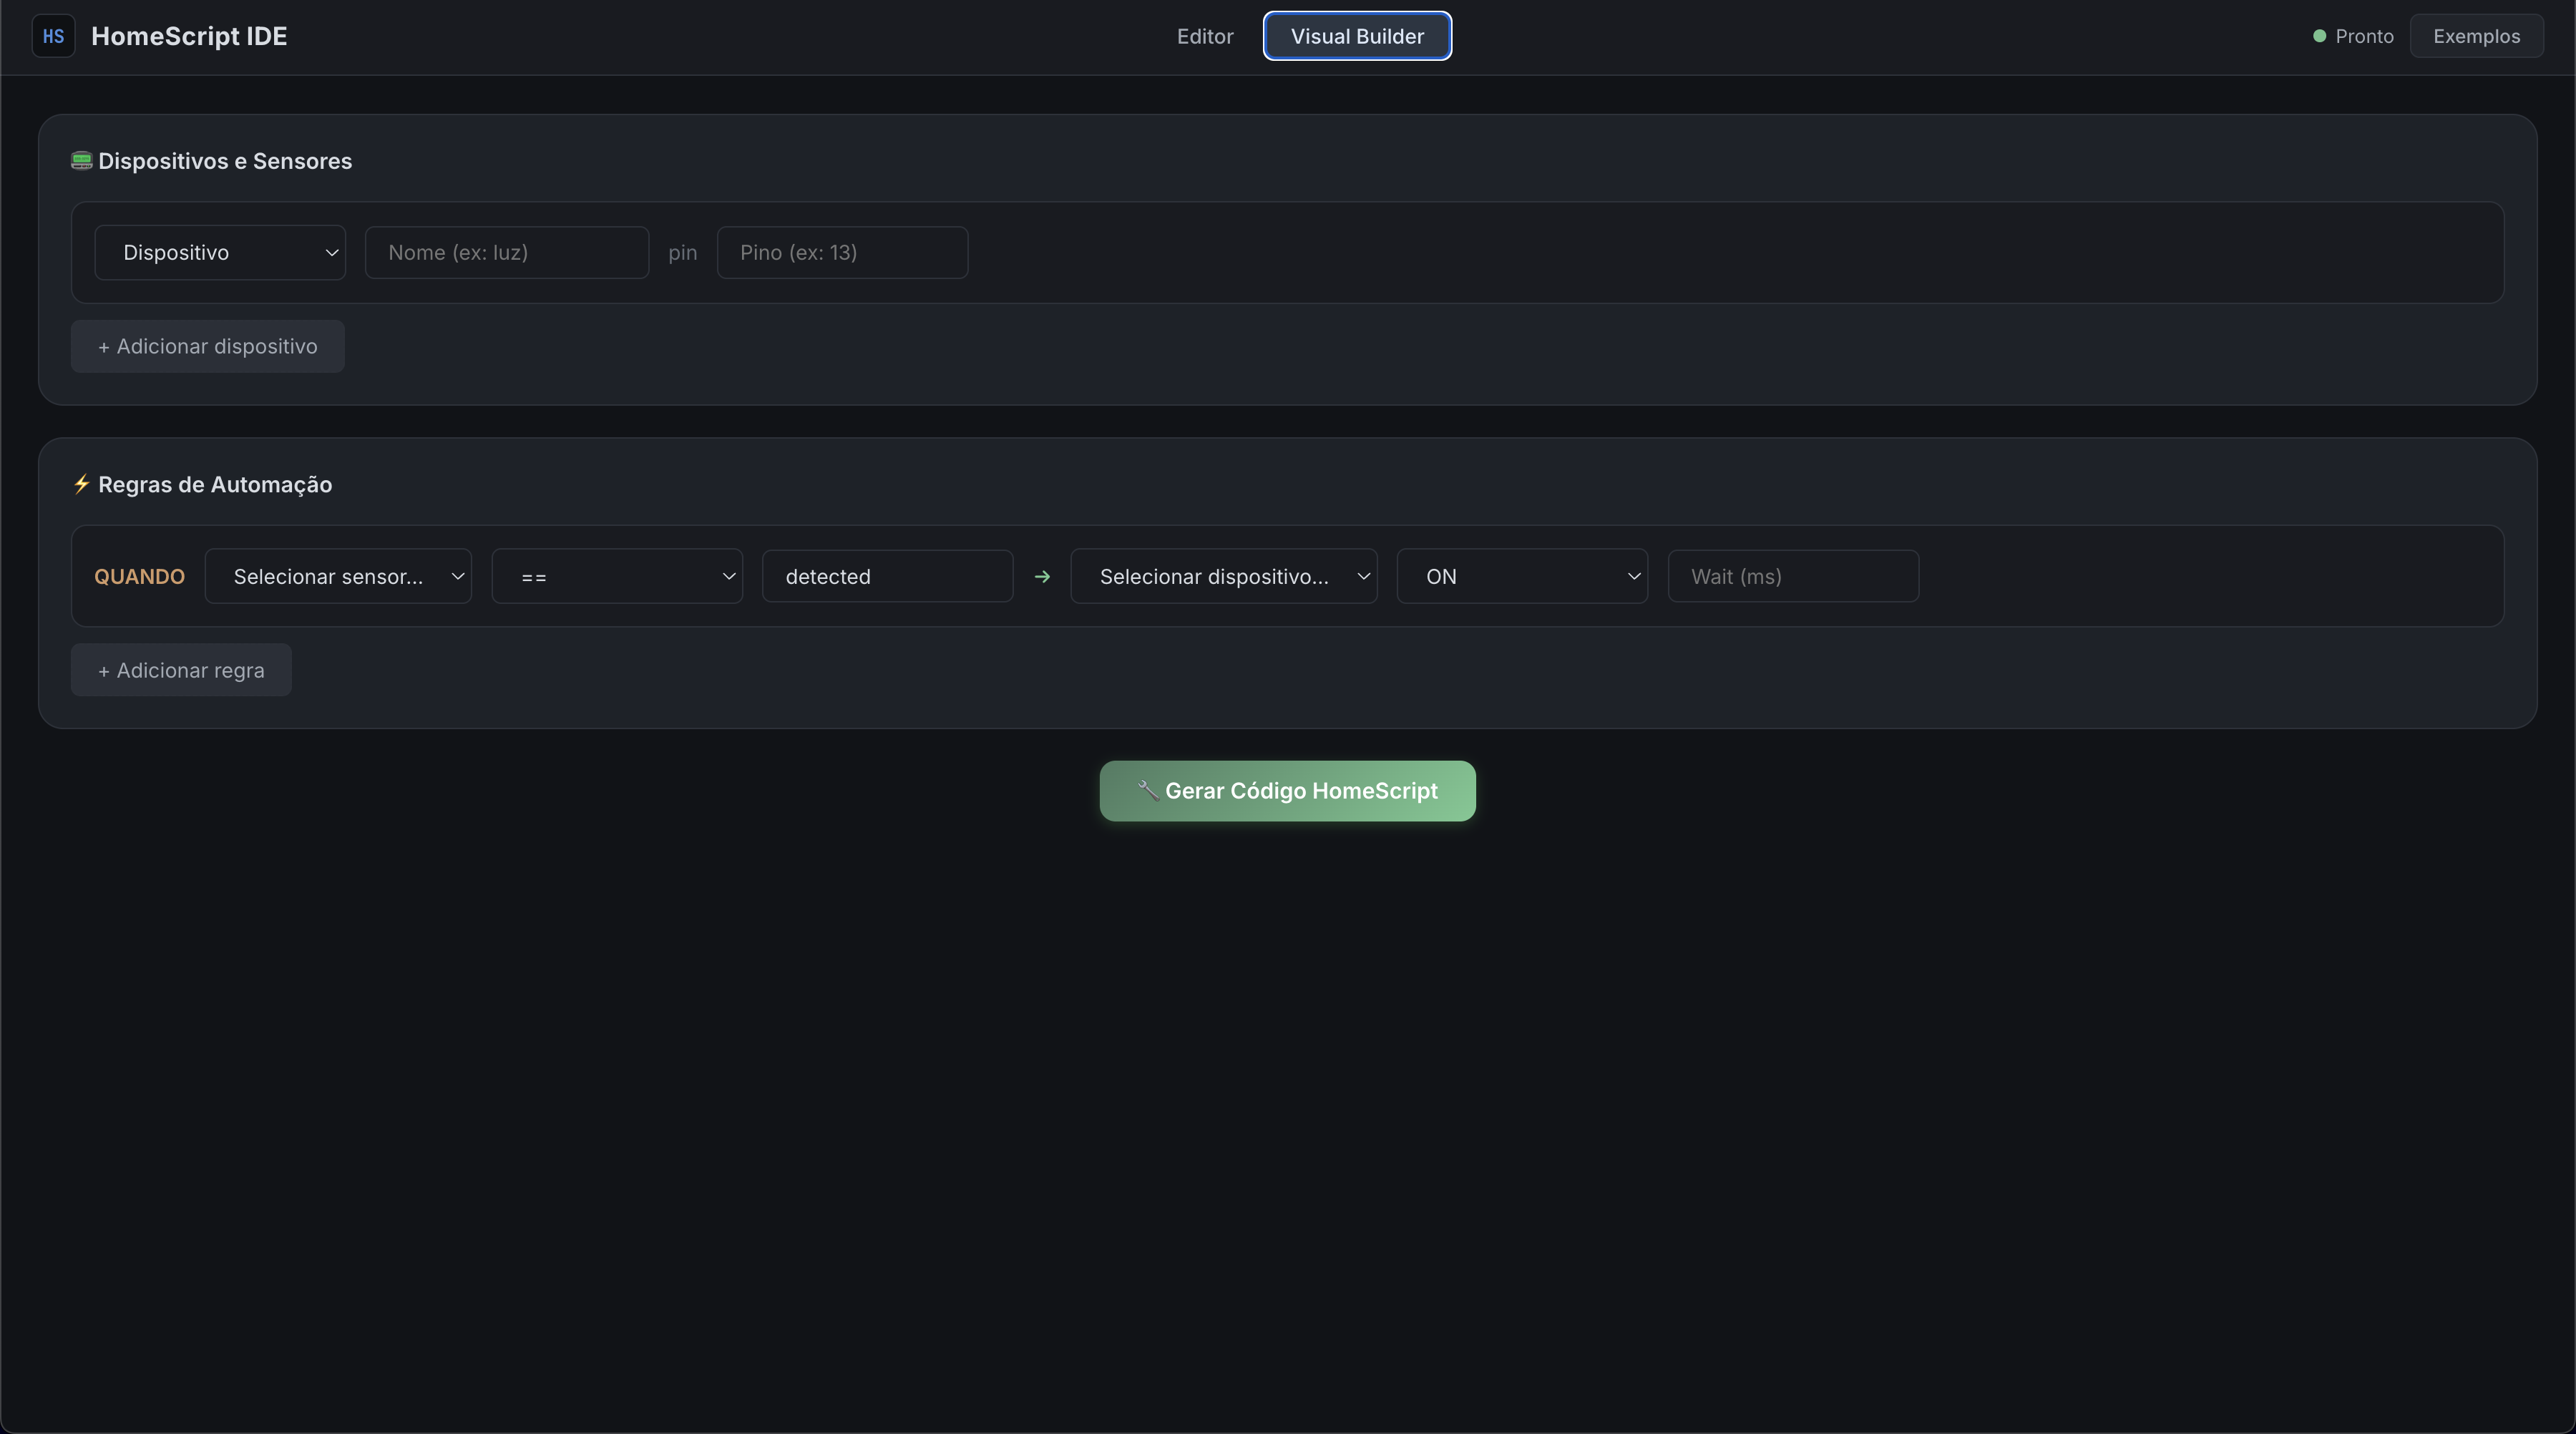
\includegraphics[width=0.95\linewidth]{../img/tela2.png}}
\caption{Visual Builder: montagem gráfica de dispositivos, sensores e regras, com geração automática de código HomeScript.}
\label{fig:visual}
\end{figure}

O repositório ainda inclui um \texttt{docker-compose.yml} que sobe os
serviços de \emph{backend} (porta 8000) e \emph{frontend} (porta 5173),
facilitando uma demonstração integrada com um único comando.

% =======================================================
\section{Validação, Resultados e Depuração}
\label{sec:validacao}

\subsection{Cenário de validação: \texttt{casa\_completa\_plus.iot}}

Para exercitar o \emph{pipeline} inteiro com um único programa, usamos o
cenário mais abrangente do repositório,
\texttt{casa\_completa\_plus.iot}, que combina \textbf{9 atuadores} e
\textbf{6 sensores} de quatro tipos distintos, variáveis, expressões
aritméticas, condicionais com \texttt{senao} aninhado, laços \texttt{para}
e \texttt{enquanto}, e telemetria serial --- e ainda mistura
deliberadamente sintaxe em inglês e português. A Tabela~\ref{tab:rotinas}
resume as seis rotinas de automação e os recursos que cada uma exercita.

\begin{table}[htbp]
\caption{Rotinas do cenário de validação e recursos exercitados}
\label{tab:rotinas}
\centering
\begin{tabular}{clp{0.44\linewidth}}
\toprule
\textbf{\#} & \textbf{Sensor/recurso} & \textbf{Recursos exercitados} \\
\midrule
1 & PIR digital & \texttt{quando/senao}, \texttt{digitalRead}, variável, \texttt{esperar} \\
2 & Reed switch & \texttt{quando/senao}, laço \texttt{para}, pulsos de buzzer \\
3 & LDR analógico & \texttt{se/senao}, \texttt{analogRead}, limiar por variável \\
4 & DHT11 & \texttt{se/senao} aninhado, cache de leitura, \texttt{isnan()} \\
5 & Potenciômetro & Sintaxe EN/PT misturada no mesmo arquivo \\
6 & HC-SR04 & \texttt{quando/senao}, \texttt{enquanto}, função auxiliar \\
\bottomrule
\end{tabular}
\end{table}

\subsection{Código C gerado: análise por rotina}
\label{subsec:codegen_analise}

O compilador transforma esse programa em código C/Arduino completo, sem
intervenção manual. O preâmbulo gerado (Listagem~\ref{lst:preambulo})
materializa cada categoria de declaração em sua forma C correspondente.

\begin{lstlisting}[style=csmall,caption={Preâmbulo e declarações globais gerados (trecho).},label={lst:preambulo}]
#include <Arduino.h>
#include <math.h>
#include <DHT.h>

#define luz_sala 13
#define luz_corredor 12
/* ... demais atuadores ... */

int movimento_sala_pin = 2;
int luminosidade_jardim_pin = A0;
int nivel_caixa_pin = A1;
DHT temperatura_quarto_dht(4, DHT11);
int distancia_garagem_trig_pin = 14;
int distancia_garagem_echo_pin = 15;

int limite_luz_jardim = 450;
int temperatura_max = 29;
/* ... demais variaveis de controle ... */
\end{lstlisting}

Para o HC-SR04, o gerador emite a função auxiliar da
Listagem~\ref{lst:hcsr04}. O \emph{timeout} de 30\,ms no \texttt{pulseIn}
evita o travamento da MCU na ausência de eco; a conversão
\texttt{duration / 58} é a aproximação inteira de
$d = \frac{t \cdot 343}{2 \times 10^{4}}$ cm, derivada da velocidade do som.

\begin{lstlisting}[style=csmall,caption={Função auxiliar gerada para o HC-SR04.},label={lst:hcsr04}]
long read_distancia_garagem_cm() {
    digitalWrite(distancia_garagem_trig_pin, LOW);
    delayMicroseconds(2);
    digitalWrite(distancia_garagem_trig_pin, HIGH);
    delayMicroseconds(10);
    digitalWrite(distancia_garagem_trig_pin, LOW);
    long duration = pulseIn(distancia_garagem_echo_pin,
                            HIGH, 30000);
    return duration / 58;
}
\end{lstlisting}

A Rotina~4 é a que melhor evidencia o gerador em ação
(Listagem~\ref{lst:rot4}). Ela demonstra três comportamentos
simultaneamente: a detecção automática do tipo DHT11 a partir do campo
\texttt{sensor\_tipo} da AST; a inserção da guarda \texttt{!isnan()} contra
leituras inválidas; e o cache de leitura, que materializa uma única
variável \texttt{leitura\_temperatura\_quarto} e a reutiliza nos dois ramos
do \texttt{if/else} aninhado, evitando uma segunda chamada custosa ao
sensor.

\begin{lstlisting}[style=csmall,caption={Rotina 4 gerada --- DHT11 com if/else aninhado e cache.},label={lst:rot4}]
float leitura_temperatura_quarto =
    temperatura_quarto_dht.readTemperature();
if (!isnan(leitura_temperatura_quarto) &&
    leitura_temperatura_quarto > temperatura_max) {
    digitalWrite(ventilador_quarto, HIGH);
    digitalWrite(aquecedor_quarto, LOW);
} else {
    if (!isnan(leitura_temperatura_quarto) &&
        leitura_temperatura_quarto < temperatura_min) {
        digitalWrite(aquecedor_quarto, HIGH);
        digitalWrite(ventilador_quarto, LOW);
    } else {
        digitalWrite(ventilador_quarto, LOW);
        digitalWrite(aquecedor_quarto, LOW);
    }
}
\end{lstlisting}

\subsection{Protótipo físico: montagem e validação}

O código C produzido pelo compilador foi gravado \emph{diretamente} em um
Arduino Uno (ATMega328P), pela IDE Arduino, sem qualquer modificação
manual. A Tabela~\ref{tab:hardware} descreve o mapeamento de pinos e
componentes do protótipo, e a Fig.~\ref{fig:arduino} mostra a montagem.

\begin{table}[htbp]
\caption{Mapeamento de pinos e componentes do protótipo físico}
\label{tab:hardware}
\centering
\begin{tabular}{p{0.33\linewidth}lc}
\toprule
\textbf{Identificador} & \textbf{Componente} & \textbf{Pino} \\
\midrule
\texttt{luz\_sala}          & LED / Relé           & 13 \\
\texttt{luz\_corredor}      & LED                  & 12 \\
\texttt{luz\_jardim}        & LED                  & 11 \\
\texttt{ventilador\_quarto} & Motor DC             & 10 \\
\texttt{aquecedor\_quarto}  & Resistor aquecedor   &  9 \\
\texttt{sirene}             & Buzzer piezoelétrico &  8 \\
\texttt{bomba\_caixa}       & Microbomba DC        &  7 \\
\texttt{portao\_motor}      & Servomotor           &  6 \\
\texttt{fita\_led\_garagem} & Fita de LEDs         &  5 \\
\texttt{movimento\_sala}    & Sensor PIR           &  2 \\
\texttt{porta\_entrada}     & Reed switch          &  3 \\
\texttt{temperatura\_quarto}& DHT11                &  4 \\
\texttt{luminosidade\_jardim}& LDR + resistor      & A0 \\
\texttt{nivel\_caixa}       & Potenciômetro        & A1 \\
\texttt{distancia\_garagem} & HC-SR04 (trig/echo)  & 14/15 \\
\bottomrule
\end{tabular}
\end{table}

\begin{figure}[htbp]
\centerline{%
\fbox{\parbox{0.9\linewidth}{\centering\vspace{1.8cm}
\textit{[Inserir foto do protótipo físico montado]}\\
Arduino Uno + 9 atuadores + 6 sensores\\
\vspace{1.8cm}}}}
\caption{Protótipo físico: Arduino Uno executando o código gerado pelo compilador HomeScript a partir de \texttt{casa\_completa\_plus.iot}.}
\label{fig:arduino}
\end{figure}

Três aspectos do código gerado foram verificados experimentalmente.
\textbf{(1)} O protocolo do HC-SR04 (Rotina~6) executou corretamente a
sequência de disparo e medição; ao aproximar a mão a menos de 35\,cm, o
\texttt{portao\_motor} acionou dois pulsos de 1.200\,ms separados por
300\,ms, reproduzindo exatamente o laço \texttt{enquanto}. \textbf{(2)} O
laço \texttt{para} com o buzzer (Rotina~2) emitiu precisamente 3 pulsos de
250\,ms ao fechar o \emph{reed switch}, confirmando a tradução correta de
inicialização, condição e incremento. \textbf{(3)} O controle térmico com
DHT11 e cache (Rotina~4) impediu o acionamento simultâneo de ventilador e
aquecedor: entre 23\,°C e 29\,°C ambos permaneceram em \texttt{LOW}; o
cache garantiu uma única leitura por ciclo. Os dados de telemetria
enviados por \texttt{Serial.println()} a 9.600 \emph{bauds} confirmaram os
valores das variáveis a cada ciclo, validando a corretude do código de
ponta a ponta --- do arquivo \texttt{.iot} ao comportamento físico
observável.

\subsection{Acertos de projeto}

Olhando o projeto em retrospecto, três decisões se mostraram acertadas. A
primeira foi \emph{manter a linguagem pequena no início}: um lexer
funcional e uma demonstração com tokens foram entregues cedo, e a partir
desse núcleo a linguagem cresceu de forma controlada. A segunda foi
\emph{produzir a saída JSON dentro do próprio compilador}, o que reduziu
drasticamente a complexidade do \emph{backend} e tornou o \emph{frontend}
um mero consumidor de dados estruturados. A terceira foi \emph{não misturar
responsabilidades}: ao manter a fonte da verdade no compilador C e proibir
qualquer análise no \emph{backend} ou no \emph{frontend}, evitou-se o risco
clássico de a CLI e a interface web divergirem de comportamento.

\subsection{Erros e depuração}

A depuração ocorreu naturalmente em camadas, refletindo a arquitetura em
fases. Erros léxicos eram investigados pelo token gerado e sua posição;
erros sintáticos, imprimindo a AST para localizar onde o \emph{parser}
parava; e código C incorreto, quase sempre, tinha origem no mapeamento da
AST para Arduino. Não por acaso, a aba de Execução do \emph{frontend}
nasceu justamente para transformar esse processo de depuração em uma
visualização. Entre os problemas concretos enfrentados estiveram:
sincronizar a gramática documentada com a implementada; preservar linha e
coluna corretas no \emph{lexer} ao avançar caracteres; representar
expressões sem construir uma árvore aritmética completa; serializar a AST
em JSON; e mapear cada tipo de sensor ao código Arduino adequado.

\subsection{Limitações}
\label{subsec:limitacoes}

Sendo honestos quanto ao alcance do trabalho, o HomeScript tem limitações
conhecidas. Os números são inteiros, não há literais de \emph{string} e os
comentários são apenas de linha. As expressões aritméticas, como
discutido, são guardadas como texto normalizado e não como subárvore, o
que impede análises mais profundas (por exemplo, avaliação de constantes).
O \emph{buffer} de código gerado tem tamanho fixo (8.192 bytes) e a
linguagem ainda não possui funções definidas pelo usuário.

Uma limitação particularmente instrutiva diz respeito à verificação de
conflito de pinos: ela é \emph{puramente lexical}, comparando os pinos como
\emph{strings}. No cenário de validação, o HC-SR04 usa \texttt{trig 14} e
\texttt{echo 15}, que no Arduino Uno correspondem fisicamente a
\texttt{A0} e \texttt{A1} --- pinos já ocupados pelos sensores
analógicos \texttt{luminosidade\_jardim} (A0) e \texttt{nivel\_caixa} (A1).
Como ``14'' e ``A0'' são \emph{strings} diferentes, o analisador semântico
não acusa o conflito, embora ele exista no hardware. Reconhecer esse caso
exigiria que o compilador modelasse a equivalência elétrica entre numeração
digital e analógica de cada placa-alvo --- um aprimoramento natural para
trabalhos futuros. Por fim, executar o compilador como subprocesso é
simples e adequado ao contexto acadêmico, mas exigiria isolamento adicional
em um ambiente de produção compartilhado.

% =======================================================
\section{Conclusão e Trabalhos Futuros}
\label{sec:conclusao}

O HomeScript demonstrou que é viável implementar, do zero e sem geradores
automáticos, um compilador completo que é, ao mesmo tempo, um exercício
acadêmico rigoroso e um esboço de produto real. A linguagem cobre um
domínio bem delimitado com sintaxe acessível e bilíngue; o compilador
percorre as quatro fases canônicas e produz código C correto para múltiplos
tipos de sensor sem intervenção do usuário; e a IDE web torna todo o
\emph{pipeline} observável e didático. A validação física com o cenário
\texttt{casa\_completa\_plus.iot} fechou o ciclo, confirmando a corretude
da tradução do arquivo \texttt{.iot} ao comportamento de 15 componentes de
hardware.

As principais contribuições técnicas foram: \textbf{(1)} um \emph{lexer}
manual com bilinguismo inglês/português no nível dos tokens; \textbf{(2)}
um \emph{parser} recursivo descendente com precedência de operadores
codificada na hierarquia de chamadas; \textbf{(3)} uma análise semântica
com tabela de símbolos, escopos e validação de tipos de sensor;
\textbf{(4)} um gerador de código com cache de leituras para sensores
lentos; e \textbf{(5)} uma IDE web com rastreamento passo a passo do
\emph{pipeline} e um construtor visual de automações.

O principal aprendizado é que a qualidade de um compilador depende tanto da
teoria das fases quanto da \emph{engenharia} ao seu redor: mensagens de
erro localizadas, formatos intermediários bem definidos (JSON) e integração
consistente entre componentes pesam tanto quanto a corretude do algoritmo
de análise. Como trabalhos futuros, destacam-se: suporte a ponto flutuante
e cadeias de caracteres; uma AST própria para expressões aritméticas;
modelagem da equivalência física de pinos por placa-alvo; geração de código
para o ESP32 com Wi-Fi e MQTT~\cite{mqtt2019}; um simulador de execução
integrado à IDE; a exportação direta de arquivos \texttt{.ino}; e o
isolamento de processos no \emph{backend} para uso em produção.

\section*{Agradecimentos}
A equipe agradece ao professor da disciplina de Linguagens Formais e
Compiladores pela orientação ao longo do projeto e pela exigência do modelo
IEEE, que guiou a organização deste relatório.

\balance
\begin{thebibliography}{00}

\bibitem{aho2006}
A.~V. Aho, M.~S. Lam, R.~Sethi, e J.~D. Ullman,
\textit{Compilers: Principles, Techniques, and Tools}, 2nd~ed.
Boston, MA: Addison-Wesley, 2006.

\bibitem{cooper2011}
K.~D. Cooper e L.~Torczon,
\textit{Engineering a Compiler}, 2nd~ed.
Burlington, MA: Morgan Kaufmann, 2011.

\bibitem{grune2012}
D.~Grune, K.~van Reeuwijk, H.~E. Bal, C.~J.~H. Jacobs, e K.~Langendoen,
\textit{Modern Compiler Design}, 2nd~ed.
New York, NY: Springer, 2012.

\bibitem{appel1998}
A.~W. Appel,
\textit{Modern Compiler Implementation in C}.
Cambridge, U.K.: Cambridge Univ. Press, 1998.

\bibitem{wirth1976}
N.~Wirth,
\textit{Algorithms + Data Structures = Programs}.
Englewood Cliffs, NJ: Prentice Hall, 1976.

\bibitem{parr2013}
T.~Parr,
\textit{The Definitive ANTLR 4 Reference}.
Raleigh, NC: Pragmatic Bookshelf, 2013.

\bibitem{kr1988}
B.~W. Kernighan e D.~M. Ritchie,
\textit{The C Programming Language}, 2nd~ed.
Englewood Cliffs, NJ: Prentice Hall, 1988.

\bibitem{mernik2005}
M.~Mernik, J.~Heering, e A.~M. Sloane,
``When and how to develop domain-specific languages,''
\textit{ACM Comput. Surv.}, vol.~37, no.~4, pp.~316--344, Dez. 2005.

\bibitem{fowler2010}
M.~Fowler,
\textit{Domain-Specific Languages}.
Boston, MA: Addison-Wesley, 2010.

\bibitem{vandeursen2000}
A.~van Deursen, P.~Klint, e J.~Visser,
``Domain-specific languages: An annotated bibliography,''
\textit{ACM SIGPLAN Notices}, vol.~35, no.~6, pp.~26--36, Jun. 2000.

\bibitem{atzori2010}
L.~Atzori, A.~Iera, e G.~Morabito,
``The Internet of Things: A survey,''
\textit{Comput. Netw.}, vol.~54, no.~15, pp.~2787--2805, Out. 2010.

\bibitem{alfuqaha2015}
A.~Al-Fuqaha, M.~Guizani, M.~Mohammadi, M.~Aledhari, e M.~Ayyash,
``Internet of Things: A survey on enabling technologies, protocols, and
applications,''
\textit{IEEE Commun. Surveys Tuts.}, vol.~17, no.~4, pp.~2347--2376, 2015.

\bibitem{gubbi2013}
J.~Gubbi, R.~Buyya, S.~Marusic, e M.~Palaniswami,
``Internet of Things (IoT): A vision, architectural elements, and future
directions,''
\textit{Future Gener. Comput. Syst.}, vol.~29, no.~7, pp.~1645--1660, 2013.

\bibitem{zanella2014}
A.~Zanella, N.~Bui, A.~Castellani, L.~Vangelista, e M.~Zorzi,
``Internet of Things for smart cities,''
\textit{IEEE Internet Things J.}, vol.~1, no.~1, pp.~22--32, Fev. 2014.

\bibitem{banzi2011}
M.~Banzi,
\textit{Getting Started with Arduino}, 2nd~ed.
Sebastopol, CA: O'Reilly Media, 2011.

\bibitem{arduino2024}
Arduino,
``Arduino Language Reference,'' 2024. [Online]. Disponível:
\url{https://www.arduino.cc/reference/en/}

\bibitem{fastapi2024}
S.~Ramírez,
``FastAPI: Modern, fast web framework for building APIs with Python,''
2024. [Online]. Disponível: \url{https://fastapi.tiangolo.com/}

\bibitem{react2024}
Meta Platforms,
``React: A JavaScript library for building user interfaces,''
2024. [Online]. Disponível: \url{https://react.dev/}

\bibitem{monaco2024}
Microsoft,
``Monaco Editor,'' 2024. [Online]. Disponível:
\url{https://microsoft.github.io/monaco-editor/}

\bibitem{mqtt2019}
OASIS Standard,
``MQTT Version 5.0,'' Mar. 2019. [Online]. Disponível:
\url{https://docs.oasis-open.org/mqtt/mqtt/v5.0/mqtt-v5.0.html}

\bibitem{docs-def}
Projeto HomeScript,
\textit{Definição da Linguagem HomeScript},
arquivo \texttt{docs/definicao\_linguagem.md}, 2026.

\bibitem{docs-tokens}
Projeto HomeScript,
\textit{Tabela de Tokens e Expressões Regulares},
arquivos \texttt{docs/tabela\_tokens.md} e \texttt{docs/regex.md}, 2026.

\end{thebibliography}

\end{document}
